\documentclass{beamer}
\usetheme[faculty=fi]{fibeamer}
\usepackage[utf8]{inputenc}
\usepackage[
  main=english, %% By using `czech` or `slovak` as the main locale
                %% instead of `english`, you can typeset the
                %% presentation in either Czech or Slovak,
                %% respectively.
  czech, slovak %% The additional keys allow foreign texts to be
]{babel}        %% typeset as follows:
%%
%%   \begin{otherlanguage}{czech}   ... \end{otherlanguage}
%%   \begin{otherlanguage}{slovak}  ... \end{otherlanguage}
%%
%% These macros specify information about the presentation
\title{Phone Shop} %% that will be typeset on the
\subtitle{Project from PA165} %% title page.
\author{Cyan Team: Martin Mejzlík, Jakub Ondrúšek, Roman Nahálka and Štefan Holečko}
%% These additional packages are used within the document:
\usepackage{ragged2e}  % `\justifying` text
\usepackage{booktabs}  % Tables
\usepackage{tabularx}
\usepackage{tikz}      % Diagrams
\usetikzlibrary{calc, shapes, backgrounds}
\usepackage{amsmath, amssymb}
\usepackage{url}       % `\url`s
\usepackage{listings}  % Code listings

\newcommand{\comment}[1]{}

\frenchspacing
\begin{document}
  \frame{\maketitle}

  \AtBeginSection[]{% Print an outline at the beginning of sections
  
  \comment{
    \begin{frame}<beamer>
      \frametitle{Outline for Section \thesection}
      \tableofcontents[currentsection]
    \end{frame}
    
  }
    }
    


  \begin{darkframes}
    \section{Phone Shop}

	\subsection{Phone Shop}
	\begin{frame}{Phone Shop}
	\framesubtitle{What is it for?}%
	  Your phone is getting old?
      \begin{itemize}
          \item shopping has never been easier
          \item quick and reliable service 24 hours a day
          \item modern and efficient
      \end{itemize}
      Our app
      \begin{itemize}
          \item simple and easy-to-use phone shop
          \item log in
          \item order a phone
          \item wait for you package
      \end{itemize}
    \end{frame}  
		
	\subsection{Function}
	\begin{frame}{Business Logic}
	\framesubtitle{What does it do?}%
        System functions
        \begin{itemize}
          \item logging on/off
          \item user administration
          \item stock administration
          \item phone administration
          \item order administration
          \item claim administration
        \end{itemize}
        System interface
        \begin{itemize}
          \item rest interface
          \item graphic interface
        \end{itemize}
    \end{frame}    
    
    \subsection{Business Logic}
	\begin{frame}{Used Technologies}
      \framesubtitle{How does it work?}%
      \begin{columns}[onlytextwidth]
      \column{.5\textwidth}
      Modules
        \begin{itemize}
          \item persistence
          \item api
          \item service
          \item spring-MVC
          \item rest
          \item ws
          \item sample data
        \end{itemize}
        \column{.5\textwidth}
        Entities
          \begin{itemize}
            \item Stock
            \item Phone 
            \item Address
            \item Person
            \item Claim
            \item Order
            \item[] 
          \end{itemize}
      \end{columns}
    \end{frame}  
    
    \subsection{Used Technologies}
	\begin{frame}{Used Technologies}
      \framesubtitle{What made it possible?}%
            \begin{tikzpicture}[overlay,remember picture]
        \node[anchor=south east,xshift=-30pt,yshift=40pt]
          at (current page.south east) {
            
\includegraphics[width=15mm]{resources/Java_programming_language_logo}
          };
      \end{tikzpicture}%
                  \begin{tikzpicture}[overlay,remember picture]
        \node[anchor=south east,xshift=-30pt,yshift=150pt]
          at (current page.south east) {
            
\includegraphics[width=35mm]{resources/Spring_Framework_Logo_2018}
          };
      \end{tikzpicture}%
      
                  \begin{tikzpicture}[overlay,remember picture]
        \node[anchor=south east,xshift=-80pt,yshift=100pt]
          at (current page.south east) {
            
\includegraphics[width=35mm]{resources/Hibernate_logo_a}
          };
      \end{tikzpicture}%
                        \begin{tikzpicture}[overlay,remember picture]
        \node[anchor=south east,xshift=-140pt,yshift=100pt]
          at (current page.south east) {
            
\includegraphics[width=35mm]{resources/junit}
          };
      \end{tikzpicture}%
                        \begin{tikzpicture}[overlay,remember picture]
        \node[anchor=south east,xshift=-130pt,yshift=40pt]
          at (current page.south east) {
            
\includegraphics[width=45mm]{resources/annotation-magic-with-mockito-mock-and-spy-lede}
          };
      \end{tikzpicture}%
      Technologies
        \begin{itemize}
          \item Java
          \item Spring
          \item Hibernate
          \item JUnit
          \item Mockito
        \end{itemize}
    \end{frame}    
    
    \subsection{User Interface}
    \begin{frame}{User Interface}
      \framesubtitle{How does it look?}%
      \begin{tikzpicture}[overlay,remember picture]
        \node[anchor=south east,xshift=-68pt,yshift=30pt]
          at (current page.south east) {
            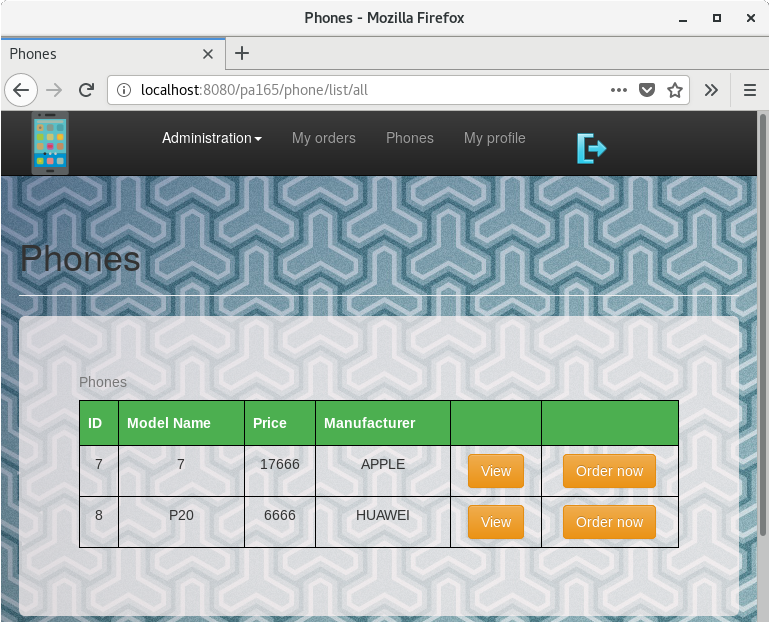
\includegraphics[width=78mm]{resources/shop}
          };
      \end{tikzpicture}%
    \end{frame}
	
	\subsection{Team Cooperation}
	\begin{frame}{Team Cooperation}
	
	Team members
        \begin{itemize}
          \item Martin
          \item Stevo
          \item Roman
          \item Kubo
        \end{itemize}
    
	\framesubtitle{Who did what?}%
	      \begin{tikzpicture}[overlay,remember picture]
        \node[anchor=south east,xshift=-40pt,yshift=150pt]
          at (current page.south east) {
            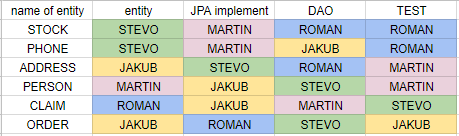
\includegraphics[width=70mm]{resources/sheetPhoneShop}
          };
      \end{tikzpicture}%
	      \begin{tikzpicture}[overlay,remember picture]
        \node[anchor=south east,xshift=-40pt,yshift=90pt]
          at (current page.south east) {
            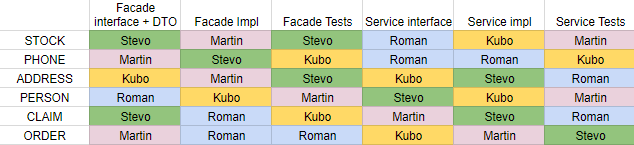
\includegraphics[width=70mm]{resources/Milestone2DivisionOfLabour}
          };
      \end{tikzpicture}%
	      \begin{tikzpicture}[overlay,remember picture]
        \node[anchor=south east,xshift=-40pt,yshift=30pt]
          at (current page.south east) {
            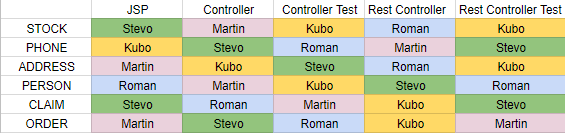
\includegraphics[width=70mm]{resources/milestone3}
          };
      \end{tikzpicture}%
    \end{frame}  
	
    
	\subsection{Feedback on PA165}
	\begin{frame}{Feedback on PA165}
	%\framesubtitle{Who did what?}%
	 
    \end{frame}  


 \subsection{Goodbye}
    \begin{frame}[plain]
    \fontsize{26pt}{0pt}\color{fibeamer@yellow}
    %\Huge
\begin{tikzpicture}[overlay, remember picture]
\node[anchor=center] at (current page.center) {

     Thank you for your attention
  };
\end{tikzpicture}
\normalsize
\end{frame}

  \end{darkframes}


\end{document}
